\fuxiti
\begin{xiaotis}

\xiaoti{$A$、$B$、$C$、$D$ 四点在同一条直线上,$AD = 50\;\haomi$, $AB = 14\;\haomi$, $CD = 18\;\haomi$, 求 $BC$ 的长。}

\begin{figure}[htbp]
    \centering
    \begin{tikzpicture}
	\tkzDefPoints{0/0/A, 1.4/0/B, 5.0/0/D, 3.2/0/C}
	\tkzDrawSegments[xianduan={below=0pt}](A,B  B,C  C,D)
	\tkzLabelPoints[above=0.3em](A,B,C,D)
\end{tikzpicture}


    \caption*{(第 1 题)}
\end{figure}


\xiaoti{测量员沿着一块地的周围测绘这块地时,
    先从点 $A$ 向北偏东 $75^\circ$ 走 240 米到点 $B$,
    再从   $B$ 向北偏西 $20^\circ$ 走 360 米到点 $C$,
    再从   $C$ 向南偏西 $65^\circ$ 走 450 米到点 $D$,
    最后从 $D$ 回到 $A$。用 1 厘来表示 100 米,画出图来,
    并量出点 $A$ 和 $D$ 的距离(精确到 10 米),以及从 $D$ 到 $A$ 的方向(精确到 $1^\circ$)。
}

\xiaoti{判断下列说法是否正确? 为什么?}
\begin{xiaoxiaotis}

    \xxt{延长直线 $AB$;}
    \xxt{延长射线 $OA$;}
    \xxt{延长线段 $AB$。}

\end{xiaoxiaotis}


\begin{enhancedline}
\xiaoti{先画线段 $AB = 20\;\haomi$, 延长 $AB$ 至 $C$, 使 $AC = 2AB$,
    在射线 $AB$ 的反向延长线上取一点 $E$,使 $AE = \exdfrac{1}{3} CE$。再计算:
}
\begin{xiaoxiaotis}

    \xxt{线段 $CE$ 的长;}
    \xxt{线段 $AC$ 是线段 $CE$ 的几分之几?}

    \xxt{线段 $CE$ 是线段 $BC$ 的几倍?}

\end{xiaoxiaotis}
\end{enhancedline}


\xiaoti{下列说法正确吗?为什么?}
\begin{xiaoxiaotis}

    \xxt{画出两点 $A$、 $B$ 的距离;}

    \xxt{已知线段 $AC$ 的长为 $10\;\limi$, 在线段 $AC$ 上画一点 $B$,使 $AB = 7\;\limi$, $BC = 4\;\limi$。}

\end{xiaoxiaotis}


\xiaoti{看图写话:}

\hspace*{2em}\begin{tblr}{column{1}={10em}}
    已知:$b > \exdfrac{c}{2}$。 & \begin{tikzpicture}
	\pgfmathsetmacro{\a}{1.0}
	\pgfmathsetmacro{\b}{1.5}
	\pgfmathsetmacro{\c}{2.0}
	\tkzDefPoints{0/0/A1, \a/0/A2, 1.3/0/B1, 1.3+\b/0/B2, 3.1/0/C1, 3.1+\c/0/C2}
	\tkzDrawSegments[xianduan={below=0pt}](A1,A2  B1,B2  C1,C2)
	\tkzLabelSegment[above](A1,A2){$a$}
	\tkzLabelSegment[above](B1,B2){$b$}
	\tkzLabelSegment[above](C1,C2){$c$}
\end{tikzpicture}

 \\
    画线段 $AD$ 等于 & \begin{tikzpicture}
	\pgfmathsetmacro{\a}{1.0}
	\pgfmathsetmacro{\b}{1.5}
	\pgfmathsetmacro{\c}{2.0}
	\pgfmathsetmacro{\xc}{\c/2}

	\tkzDefPoints{0/0/A, \a/0/E, \a+\a/0/B, \a+\a+\b/0/C, \a+\a+\b-\xc/0/D, \a+\a+\b+0.5/0/M}
	\tkzDrawSegment(A,M)
	\tkzDrawSegments[xianduan={above=3pt, below=0pt}](A,E  E,B  B,C)
	\tkzDrawSegments[dim={$a$,-1em,}](A,E)
	\tkzDrawSegments[dim={$a$,-1em,}](E,B)
	\tkzDrawSegments[dim={$b$,-1em,}](B,C)
	\tkzDrawSegments[dim={$\dfrac{c}{2}$,1em,}](D,C)
	\tkzLabelPoints[above=0.3em](A)
	\tkzLabelPoints[above=0.3em, xshift=-0.5em](D)
\end{tikzpicture}

 \\
\end{tblr}

\hspace*{2em}\begin{tblr}{column{1}={10em}}
    画法:(1) & \begin{tikzpicture}
	\pgfmathsetmacro{\a}{1.0}
	\pgfmathsetmacro{\b}{1.5}
	\pgfmathsetmacro{\c}{2.0}
	\pgfmathsetmacro{\xc}{\c/2}

	\tkzDefPoints{0/0/A, 0/0.1/pa, \a/0/E, \a+\a/0/B, \a+\a+\b/0/C, \a+\a+\b-\xc/0/D, \a+\a+\b+0.5/0/M}
	\tkzDrawSegment(A,M)
	\tkzDrawSegment(A,pa)
	\tkzLabelPoints[above=0.3em](A)
	\tkzLabelPoints[above](M)
\end{tikzpicture}

 \\
    (2) & \begin{tikzpicture}
	\pgfmathsetmacro{\a}{1.0}
	\pgfmathsetmacro{\b}{1.5}
	\pgfmathsetmacro{\c}{2.0}
	\pgfmathsetmacro{\xc}{\c/2}

	\tkzDefPoints{0/0/A, 0/0.1/pa, \a/0/E, \a+\a/0/B, \a+\a+\b/0/C, \a+\a+\b-\xc/0/D, \a+\a+\b+0.5/0/M}
	\tkzDrawSegment(A,M)
	\tkzDrawSegment(A,pa)
	\tkzLabelPoints[above=0.3em](A)
	\tkzLabelPoints[above](M)

	\tkzDrawSegments[dim={$a$,-1em,}](A,E)
	\tkzDrawSegments[dim={$a$,-1em,}](E,B)
	\tkzLabelPoints[above=0.3em](B)
\end{tikzpicture}

 \\
    (3) & \begin{tikzpicture}
	\pgfmathsetmacro{\a}{1.0}
	\pgfmathsetmacro{\b}{1.5}
	\pgfmathsetmacro{\c}{2.0}
	\pgfmathsetmacro{\xc}{\c/2}

	\tkzDefPoints{0/0/A, 0/0.1/pa, \a/0/E, \a+\a/0/B, \a+\a+\b/0/C, \a+\a+\b-\xc/0/D, \a+\a+\b+0.5/0/M}
	\tkzDrawSegment(A,M)
	\tkzDrawSegment(A,pa)
	\tkzLabelPoints[above=0.3em](A)
	\tkzLabelPoints[above](M)

	\tkzDrawSegments[xianduan={above=3pt, below=0pt}](A,E  E,B  B,C)
	\tkzDrawSegments[dim={$b$,-1em,}](B,C)
	\tkzLabelPoints[above=0.3em](B,C)
\end{tikzpicture}

 \\
    (4) & \begin{tikzpicture}
	\pgfmathsetmacro{\a}{1.0}
	\pgfmathsetmacro{\b}{1.5}
	\pgfmathsetmacro{\c}{2.0}
	\pgfmathsetmacro{\xc}{\c/2}

	\tkzDefPoints{0/0/A, 0/0.1/pa, \a/0/E, \a+\a/0/B, \a+\a+\b/0/C, \a+\a+\b-\xc/0/D, \a+\a+\b+0.5/0/M}
	\tkzDrawSegment(A,M)
	\tkzDrawSegment(A,pa)
	\tkzLabelPoints[above=0.3em](A)
	\tkzLabelPoints[above](M)

	\tkzDrawSegments[xianduan={above=3pt, below=0pt}](A,E  E,B  B,C  D,C)
	\tkzDrawSegments[dim={$\dfrac{c}{2}$,-1em,}](D,C)
	\tkzLabelPoints[above=0.3em](B,C,D)
\end{tikzpicture}

 \\
\end{tblr}


\xiaoti{画 $\angle A = 50^\circ$,在 $\angle A$ 的两边上分别取 $B$、$C$ 两点,
    使 $AB = 35\;\haomi$,$AC = 30\;\haomi$, 连结 $BC$。
    (1) 量 $BC$ 的长(精确到 $1\;\haomi$);
    (2) 量 $\angle ABC$ 和 $\angle BCA$ 的度数(精确到 $1^\circ$),
    并计算 $\angle A + \angle ABC + \angle BCA$ 的度数和。
}


\xiaoti{画 $AB = 60\;\haomi$, $\angle DAB = 35^\circ$, $\angle EBA = 44^\circ$, $AD$ 和 $BE$ 相交于 $C$。
    画 $\angle CAB$、 $\angle ABC$、 $\angle BCA$ 的平分线。
}

\xiaoti{计算:}
\begin{xiaoxiaotis}

    \xxt{$77^\circ 42' + 32^\circ 30' + 69^\circ 48'$;}

    \xxt{$180^\circ - 46^\circ 37' 45'' - 65^\circ 28' 30''$;}

    \xxt{$18^\circ 43' 26'' \times 5$;}

    \xxt{$360^\circ \div 7$(精确到 $1'$)。}

\end{xiaoxiaotis}


\xiaoti{已知直线 $AB$、$CD$ 相交于点 $O$,用量角器画各角的平分线 $OE$、 $OH$、 $OG$、 $OF$,
    并计算 $\angle EOH$, $\angle HOG$。 $E$、$O$、$G$ 三点在一条直线上吗?
}

\begin{figure}[htbp]
    \centering
    \begin{tikzpicture}
	\tkzDefPoints{-2/1.5/A, 2/-1.5/B, 2/2/C, -2/-2/D}
	\tkzInterLL(A,B)(C,D)   \tkzGetPoint{O}
	\tkzDefLine[bisector](A,O,D) \tkzGetPoint{E}
	\tkzDefLine[bisector](B,O,C) \tkzGetPoint{G}
	\tkzDefLine[bisector](A,O,C) \tkzGetPoint{H}
	\tkzDefLine[bisector](B,O,D) \tkzGetPoint{F}

	\tkzDrawSegments(A,B  C,D)
	\tkzDrawSegments[dashed](E,G)
	\tkzDrawSegments[dashed](H,F)
	\tkzLabelPoints[left](A)
	\tkzLabelPoints[right](C,H)
	\tkzLabelPoints[below](D,F,B, E,G)
	\tkzLabelPoints[below=0.5em, xshift=-0.5em](O)
\end{tikzpicture}


    \caption*{(第 10 题)}
\end{figure}


\xiaoti{判断正误,错误的加以改正:}
\begin{xiaoxiaotis}

    \xxt{在 $\angle ABC$ 的一边的延长线上取一点 $D$;}

    \xxt{两条射线组成的图形叫做角;}

    \xxt{$\angle B = \angle ABC + \angle CBD$。}

\end{xiaoxiaotis}


\xiaoti{把一个平角三等分,求两旁两角的平分线所成的角的度数。}

\xiaoti{一个角的补角等于这个角的余角的 4 倍,画这个角。}

\xiaoti{已知 $\angle \alpha$ 和 $\angle \beta$ 互为补角,并且 $\angle \alpha$ 比 $\angle \beta$ 大 $30^\circ$,
    求 $\angle \alpha$ 和 $\angle \beta$ 的大小。
}

\xiaoti{已知:$\angle AOB$ 与 $\angle BOC$ 是邻补角,$OD$ 是 $\angle AOB$ 的角平分线, $OE$ 是 $\angle BOC$ 的平分线。}
\begin{xiaoxiaotis}

    \xxt{画出它们的图形;}

    \xxt{求 $\angle DOE$ 的大小;}

    \xxt{指出 $\angle BOE$ 的余角;}

    \xxt{指出 $\angle EOC$ 的余角、补角、邻补角。}

\end{xiaoxiaotis}

\end{xiaotis}

